\documentclass[11pt]{article}

\usepackage[preprint]{acl}

\usepackage{times}
\usepackage{latexsym}
\usepackage[T1]{fontenc}
\usepackage[utf8]{inputenc}
\usepackage{microtype}
\usepackage{inconsolata}
\usepackage{graphicx}
\usepackage{booktabs}
\usepackage{amsmath}
\usepackage{amssymb}
\usepackage{amsfonts}
\usepackage{multirow}
\usepackage{array}
\usepackage{float}
\usepackage{xcolor}
\usepackage{tikz}
\usepackage{pgf}
\usetikzlibrary{arrows.meta,shapes.geometric,positioning,fit,backgrounds,calc}

\newcolumntype{L}[1]{>{\raggedright\arraybackslash}m{#1}}
\newcolumntype{C}[1]{>{\centering\arraybackslash}m{#1}}
\newcommand{\tablebodyfont}{\normalsize\setlength{\tabcolsep}{3pt}\renewcommand{\arraystretch}{1.12}}
\newcommand{\displaynote}[1]{%
  \vspace{0.25em}
  \parbox{\linewidth}{\raggedright\normalsize\textit{Note.} #1}%
}
\newcommand{\promptbox}[1]{%
  \begin{center}
  \setlength{\fboxsep}{8pt}%
  \noindent\fbox{%
    \parbox{0.94\linewidth}{%
      \raggedright\ttfamily\normalsize
      #1
    }%
  }
  \end{center}
}
\newcommand{\examplebox}[8]{%
  \begingroup
  \setlength{\fboxsep}{8pt}%
  \noindent\fbox{%
    \begin{minipage}{0.96\linewidth}
    \textbf{#1}\par\vspace{0.5em}
    \begin{minipage}[t]{0.25\linewidth}
    \vspace{0pt}\centering
    \includegraphics[width=0.96\linewidth]{#2}
    \end{minipage}\hfill
    \begin{minipage}[t]{0.69\linewidth}
    \vspace{0pt}\raggedright
%   \texttt{example\_id}: \texttt{\detokenize{#3}}\\
%   \texttt{image\_file}: \texttt{\detokenize{#4}}\\
    \textbf{Caption:} #5\par
    \textbf{Question:} #6\par
    \textbf{Gold answer:} #7\par
    \textbf{Oracle action:} \texttt{\detokenize{#8}}.
    \end{minipage}
    \end{minipage}%
  }
  \endgroup
}

% Citation key aliases:
% liBLIP2BootstrappingLanguageImage2023, liuVisualInstructionTuning2023,
% daiInstructBLIPGeneralpurposeVisionLanguage2023, huaHowVisionLanguageModels2025,
% popordanoskaCLASHBenchmarkCrossModal2025, zhangRobustMultimodalLarge2025,
% zhangEvaluatingSteeringModality2025, wenKnowYourLimits2025,
% zhangWhenModalitiesConflict2025, zhangInstructionAnchorsDissecting2026,
% jiaSeeingSoundHearing2025, liEvaluatingObjectHallucination2023,
% faveroMultiModalHallucinationControl2024, sethSystematicEvaluationHallucinations2025,
% yanMultimodalInconsistencyReasoning2025, chenSurveyMultimodalHallucination2025,
% qwen25vl_2025, antol_vqa_2015, goyal_vqav2_2017

\title{When Senses Disagree: Conflict-Aware Arbitration for\\Multimodal Reasoning}

\author{Otto Xin \\
  Department of Communication Studies \\
  Northwestern University \\
  Evanston, IL 60208 \\
  \texttt{haohangxin@u.northwestern.edu} \\\And
  Nicholas Ornstein \\
  Department of Communication Studies \\
  Northwestern University \\
  Evanston, IL 60208 \\
  \texttt{nickornstein@u.northwestern.edu}}

\begin{document}

\maketitle

\begin{abstract}
Multimodal large language models (MLLMs) are brittle when image and text inputs disagree: instead of recognizing conflict, they often answer confidently with information from the wrong modality. We frame this as an arbitration problem, where a model must determine whether each modality is informative and whether informative modalities agree. We propose \textbf{CARM} (Conflict-Aware Reasoning Module), a lightweight module for frozen MLLMs that predicts modality informativeness, cross-modal relation, and a final action in a staged cascade. We evaluate CARM on Conflict Suite, a 44,948-example benchmark built from VQAv2/COCO under a five-category conflict protocol. On the canonical full split (31,463 train / 6,743 validation / 6,742 test) with Qwen2.5-VL-7B, CARM reaches 66.2\% task success on the test set, improving over the strongest non-learned baseline from 48.9\% to 66.2\%. A full-data ablation shows that hidden-state features account for most of the gain, while the cascade adds a smaller further improvement from 65.1\% to 66.2\% over a flat hidden-state control. These results suggest that multimodal conflict handling is better modeled as explicit arbitration than as generic abstention or confidence estimation.
\end{abstract}


\section{Introduction}
\label{sec:intro}

Multimodal large language models (MLLMs) are attractive because they can combine images and
language in a single reasoning pipeline, but they become unreliable when those modalities
disagree. In realistic deployments, such disagreements are common: captions can be stale,
retrieved text can describe the wrong image, and one modality can be ambiguous while the
other is decisive. In these cases, current MLLMs often produce fluent but evidentially
ungrounded answers instead of acknowledging that the modalities conflict or that one of
them should be ignored~\citep{huaHowVisionLanguageModels2025,popordanoskaCLASHBenchmarkCrossModal2025,zhangRobustMultimodalLarge2025,dengWordsVisionVisionLanguage2025,yanMultimodalInconsistencyReasoning2025}.

The key difficulty is that conflict handling is a structured decision problem, not just a
generic uncertainty problem. A system must determine whether the image is informative for
the question, whether the text is informative, and, if both are informative, whether the
two modalities agree. Existing mitigations typically operate at the wrong level of
abstraction. Prompting-based verification and generic abstention heuristics can reduce some
errors, but they do not explicitly model the arbitration structure of the problem
itself~\citep{zhangEvaluatingSteeringModality2025,wenKnowYourLimits2025}. This leads to
two familiar mistakes: over-commitment when both modalities are confident but contradictory,
and over-abstention when only one modality is useful.

We address this gap with CARM (Conflict-Aware Reasoning Module), a lightweight module that attaches to a frozen MLLM
backbone and makes the arbitration structure explicit. Our central empirical observation is
that, for Qwen2.5-VL-7B, last-layer hidden states from the full multimodal pass provide a
much stronger arbitration signal than output distributions alone. CARM therefore combines
two unimodal probes with hidden-state features from the joint pass, then predicts modality
informativeness, cross-modal relation, and final action in a three-stage cascade.

\paragraph{Contributions.}
This paper makes three contributions. First, we formalize multimodal conflict handling as a
five-category protocol with oracle actions and evaluate it on our 'Conflict Suite,' a balanced
benchmark built from VQAv2 and MSCOCO. Second, we introduce CARM, a frozen-backbone cascade that
separates modality informativeness, cross-modal relation, and action selection. Third, on
this controlled Qwen2.5-VL-7B testbed and the canonical full split, we show that the resulting
structure improves final decision quality: CARM reaches 66.2\% task success on a 6,742-example
test split, improving on the strongest non-learned baseline from 48.9\% to 66.2\%, and our
ablations show that hidden-state inputs are the main source of the gain while the cascade
itself raises task success from 65.1\% to 66.2\% over a flat hidden-state control.


\section{Related Work}
\label{sec:related}

\paragraph{Conflict and hallucination in MLLMs.}
Modern MLLMs connect a pretrained vision encoder to a language model through a learned
cross-modal interface~\citep{liBLIP2BootstrappingLanguageImage2023,liuVisualInstructionTuning2023,daiInstructBLIPGeneralpurposeVisionLanguage2023}.
Although these systems perform well on aligned inputs, they remain brittle when image and
text disagree, often hallucinating from the wrong modality or failing to ground their final
answer~\citep{liEvaluatingObjectHallucination2023,faveroMultiModalHallucinationControl2024,sethSystematicEvaluationHallucinations2025}.
Recent surveys frame this as part of a broader multimodal hallucination and reliability
problem, and related work also studies cross-modality knowledge conflict as a distinct
failure source~\citep{chenSurveyMultimodalHallucination2025,zhuUnravelingCrossModalityKnowledge2024}.
Our work focuses on this input-conflict failure mode directly.

\paragraph{Benchmarks and modality bias.}
Recent benchmarks make modality conflict measurable at scale. CLASH introduces controlled
object- and attribute-level contradictions~\citep{popordanoskaCLASHBenchmarkCrossModal2025},
while MMIR extends inconsistency evaluation to layout-rich artifacts such as webpages,
slides, and posters~\citep{yanMultimodalInconsistencyReasoning2025}. Subsequent
evaluations show that conflict degrades performance even when each modality is individually
informative~\citep{zhangRobustMultimodalLarge2025}. Related work also documents strong
modality bias and instance-dependent dominance in multimodal systems, including cases where
models over-trust text under inconsistency~\citep{huaHowVisionLanguageModels2025,zhangWhenModalitiesConflict2025,jiaSeeingSoundHearing2025,dengWordsVisionVisionLanguage2025}.
Mechanistic analyses further suggest that arbitration behavior is reflected in latent
representations and specialized internal components rather than only in final outputs
~\citep{zhangEvaluatingSteeringModality2025,zhangInstructionAnchorsDissecting2026}.
Unlike work that only diagnoses the failure, we cast conflict resolution as a structured
action-selection problem.

\paragraph{Abstention and selective prediction.}
Selective prediction trades coverage for risk by abstaining on examples where a model is
likely to err~\citep{geifmanSelectiveClassificationDeep2017,kamathSelectiveQuestionAnswering2020,wenKnowYourLimits2025}.
In VQA, reliable-answering work shows that simple confidence thresholding can achieve low
risk only at very low coverage~\citep{whiteheadReliableVisualQuestion2022}. Multimodal
conflict requires a more structured decision: a system should abstain for different reasons
in contradictory and both-weak cases, while still answering when exactly one modality is
informative. CARM addresses this by predicting modality informativeness, the congruence or incongruence of the implied answers of each modality to the target question, and
final action, explicitly rather than learning a single abstention threshold.


\section{Task Setting}
\label{sec:task}

\paragraph{Decision problem.}
Given image $I$, text caption $T$, and question $q$, the system predicts an action
$\hat{a}$ and, when appropriate, an answer $\hat{y}$. We use four actions:
\texttt{trust\_vision}, \texttt{trust\_text}, \texttt{require\_agreement}, and
\texttt{abstain}. A correct decision depends on two modality-specific properties
(whether vision and text are informative for $q$) and one pairwise property
(whether the informative modalities agree).

\paragraph{Five-category protocol.}
Table~\ref{tab:protocol} summarizes the protocol we developed to evaluate these possible behaviors. Category 1 (C1) and Category 4 (C4) are scenarios where both modalities contained relevant information with which to answer the question; they differ only in whether those modalities are consistent over the question (C1) or inconsistent (C4). C2 and C3 are asymmetric single-modality cases, and C5 captures the case where the answer-relevant signal in both modalities is unclear.

\begin{table}[t]
\centering
\caption{Conflict protocol categories and oracle actions. Each category is defined by the
cross-product of per-modality informativeness and pairwise consistency, with a
deterministic oracle action.}
\label{tab:protocol}
\tablebodyfont
\begin{tabular*}{\linewidth}{@{\extracolsep{\fill}}L{0.08\linewidth}C{0.15\linewidth}C{0.15\linewidth}C{0.26\linewidth}C{0.24\linewidth}@{}}
\toprule
Cat. & \shortstack{Vision\\info.?} & \shortstack{Text\\info.?} & Relation & Oracle action \\
\midrule
C1 & yes & yes & consistent & require agreement \\
C2 & yes & no & --- & trust vision \\
C3 & no & yes & --- & trust text \\
C4 & yes & yes & contradictory & abstain \\
C5 & no & no & --- & abstain \\
\bottomrule
\end{tabular*}
\end{table}


\paragraph{Conflict Suite construction and evaluation.}
We build a "Conflict Suite" from VQAv2/COCO~\citep{antol_vqa_2015,goyal_vqav2_2017}
and assign protocol labels programmatically from modality-specific supervision fields
derived with the Qwen2.5-VL-7B backbone. The resulting corpus contains 44,948 examples and
is nearly balanced across C1--C5. Unless otherwise noted, we report results on the
canonical prepared split: 31,463 training examples, 6,743 validation examples, and
6,742 test examples.
We use VQAv2/COCO because it offers controlled answer supervision and reproducible conflict
construction at scale; complementary reliability benchmarks such as POPE, CLASH, and MMIR
target hallucination or contradiction detection, but not the full five-way arbitration
decision studied here~\citep{liEvaluatingObjectHallucination2023,popordanoskaCLASHBenchmarkCrossModal2025,yanMultimodalInconsistencyReasoning2025}.
Appendix~\ref{app:dataset} reports the exact corpus and split counts used in the main
comparison.

Dataset construction required systematic perturbation of the inconsistent modality. In the initial joined VQA + MSCOCO state, generally, both the caption and the image contained the information necessary to answer the question. This corresponded to a Category 1 type scenario in our taxonomy. To create Category 2 scenarios, where the caption did not answer the question (but otherwise was similar) we processed all C2 captions by passing them to an LLM-as-annotator (GPT-5-nano) and instructing the model to change the caption so it no longer answered the question (for example, removed the word "red" from the caption when the question asks for the color). Upon inspection, this was highly effective. 

To build C3, we needed to change images so they no longer answered the question. To achieve this, we leveraged the fact that the COCO images have existing object annotations, for objects across the 80 COCO categories (e.g., [person, tennis racket]). We first limited the question-image-caption-answer scenarios to only those where the COCO annotated object appears verbatim in the question, so that it is likely the question is asking about the COCO object (i.e., ["tennis racket"] is in the question). Then, we embedded all images not yet included in the dataset, as well as the target image, using CLIP embeddings. Then, after excluding all images that also contained the target image's COCO objects (so none with a tennis racket) we selected the closest image in embedding space and swapped it in. Thus, it likely was similar to the original (close in embedding space) but lacked an object in the question, and thus could not be used to answer the question.

Category 4, which required contradicting implied answers from caption and image, used the text perturbation approach with GPT-5-nano, except asking the LLM to change the answer the question implied. There was no need to perturb the image as contradiction is symmetric, and there was no longer a "golden" answer at all.

Category 5 was constructed by swapping images as before, and perturbing text for irrelevance (not difference), as before. These dataset construction methods allowed us to cover the range of modality conflict scenarios that we hoped to test.

\paragraph{Metrics.}
Our primary metric is task success (TS): a prediction succeeds only if it takes
the right arbitration action and, on answerable categories, returns the correct answer.
This makes abstention correct for C4/C5 and correct answering necessary for C1--C3. We
also report action accuracy, coverage (the fraction of examples on which
the system answers), and accuracy-on-answered (AoA). Under this definition, the protocol
oracle achieves TS $= 1.0$ by construction. Because that ceiling is definitionally built
into the protocol, Appendix~\ref{app:analysis} also reports a practical fixed-output
ceiling: under the same four protocol actions and frozen probe outputs, an oracle router
would reach 89.5\% task success on this full test split. CARM therefore captures 74.0\%
of the attainable task success under the operational ceiling induced by the frozen
backbone outputs. Appendix~\ref{app:dataset} gives the exact task-success rule and
representative cases, and Appendix~\ref{app:eval-details} reports the full evaluation
tables.


\section{CARM}
\label{sec:method}

\subsection{Overview}

Arbitrating between conflicting modalities requires three kinds of evidence: a signal for
whether vision is useful, a signal for whether text is useful, and a signal for whether the
two modalities agree when both matter. CARM extracts these signals from a frozen
Qwen2.5-VL-7B backbone and then maps them to an action with a small cascade of prediction
heads. Figure~\ref{fig:arch} shows the full pipeline.

\begin{figure}[t]
\centering
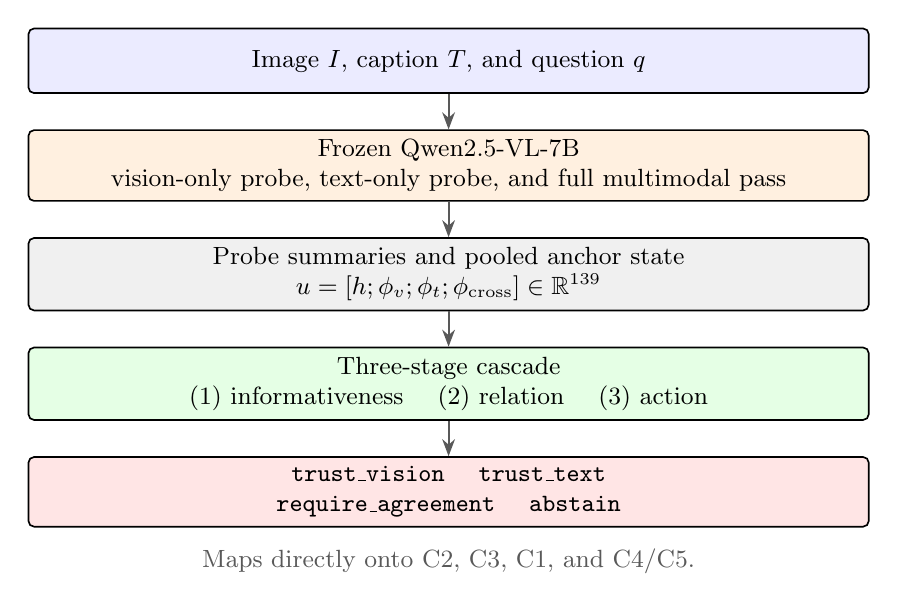
\begin{tikzpicture}[
  font=\small,
  >=Stealth,
  node distance=0.45cm,
  box/.style={draw, rounded corners=2pt, minimum height=0.82cm,
              minimum width=0.88\columnwidth, align=center, line width=0.6pt},
  inputbox/.style={box, fill=blue!8},
  featbox/.style={box, fill=orange!12},
  stagebox/.style={box, fill=green!10},
  actionbox/.style={box, fill=red!10},
  trunkbox/.style={box, fill=gray!12},
  arrow/.style={->, line width=0.7pt, color=gray!70!black},
  note/.style={font=\small, text=gray!70!black, align=center},
]
\node[inputbox] (input) {Image $I$, caption $T$, and question $q$};
\node[featbox, below=of input] (queries)
  {Frozen Qwen2.5-VL-7B\\vision-only probe, text-only probe, and full multimodal pass};
\node[trunkbox, below=of queries] (features)
  {Probe summaries and pooled anchor state\\$u=[h;\phi_v;\phi_t;\phi_{\mathrm{cross}}] \in \mathbb{R}^{139}$};
\node[stagebox, below=of features] (cascade)
  {Three-stage cascade\\(1) informativeness \quad (2) relation \quad (3) action};
\node[actionbox, below=of cascade] (actions)
  {\texttt{trust\_vision} \quad \texttt{trust\_text}\\\texttt{require\_agreement} \quad \texttt{abstain}};
\node[note, below=0.15cm of actions] {Maps directly onto C2, C3, C1, and C4/C5.};

\draw[arrow] (input) -- (queries);
\draw[arrow] (queries) -- (features);
\draw[arrow] (features) -- (cascade);
\draw[arrow] (cascade) -- (actions);

\end{tikzpicture}
\caption{CARM architecture. CARM keeps the backbone frozen, extracts unimodal and
cross-modal evidence, and makes a staged arbitration decision.}
\label{fig:arch}
\end{figure}


\subsection{Features from a Frozen Backbone}

Arbitration requires evidence about each modality separately and jointly. We therefore run
three backbone passes: a vision-only probe, a text-only probe, and a full multimodal pass.
The probe distributions are defined over a small family-specific VQA vocabulary selected by
question type. In the reported Qwen2.5-VL-7B runs, this vocabulary is fixed by the backbone
configuration rather than mined from the training split: existence uses \{yes, no,
unknown\}, count uses integers 0--20 plus \texttt{unknown}, and attribute-color uses 11
canonical color labels plus \texttt{unknown}. Appendix~\ref{app:vocab-details} gives the
exact ontology and canonicalization details. The full multimodal pass yields a fixed-width anchor-state
sequence from the last hidden layer of the multimodal prompt. We summarize each probe with
entropy, top-two margin, and max probability, add a small set of agreement features, and
concatenate those summaries with the mean-pooled 128-dimensional anchor-state vector:
\[
u = [h;\phi_v;\phi_t;\phi_{\text{cross}}] \in \mathbb{R}^{139}.
\]
This combines lightweight confidence signals with a richer joint representation that is not
available from output probabilities alone. Appendix~\ref{app:method-details} gives the
exact formulas and prompt templates.

\subsection{Cascade Arbitration}

A flat action classifier would conflate decisions with different prerequisites. Choosing
\texttt{trust\_vision} or \texttt{trust\_text} requires knowing which modality is
informative, while abstaining in C4 requires knowing that both modalities are informative
and contradictory. CARM mirrors that logic with a three-stage cascade over a shared
128-dimensional trunk. Stage~1 predicts vision and text informativeness, Stage~2 predicts
the cross-modal relation (consistent, contradictory, asymmetric, or both-weak), and
Stage~3 predicts the final action conditioned on the earlier stages. In asymmetric cases,
the final head uses the Stage~1 informativeness predictions to choose between
\texttt{trust\_vision} and \texttt{trust\_text}. We train all
stages jointly while keeping the backbone strictly frozen. This keeps the decision process
auditable and adds only 36,236 trainable parameters relative to the 7B backbone.

\subsection{Training Objective}
\label{sec:training-objective}

We train CARM against the explicit arbitration structure rather than only the final action.
Each example provides supervision for vision informativeness, text informativeness,
pairwise relation, and final action. For Cascade CARM, we optimize the weighted multi-task
objective:
\begin{align*}
\mathcal{L}
&= \lambda_v\,\mathrm{CE}(\hat{l}_v, l_v)
+ \lambda_t\,\mathrm{CE}(\hat{l}_t, l_t) \\
&\quad + \lambda_r\,\mathrm{CE}(\hat{l}_{\mathrm{rel}}, l_{\mathrm{rel}})
+ \lambda_a\,\mathrm{CE}(\hat{l}_{\mathrm{act}}, l_{\mathrm{act}}).
\end{align*}
This objective encourages the model to learn the intermediate arbitration decisions that
lead to the final action, instead of collapsing the whole problem into a single flat label.
The distribution variants use the same staged objective with distribution inputs in place of
hidden-state inputs, while Flat Hidden keeps only the final action loss and removes the
auxiliary heads. Exact loss weights and optimization settings are given in
Section~\ref{sec:experiments} and Appendix~\ref{app:method-details}.


\section{Experimental Setup}
\label{sec:experiments}

We evaluate on the canonical full split of Conflict Suite (31,463 training, 6,743
validation, and 6,742 test examples). Appendix~\ref{app:dataset} reports the exact corpus
counts, split construction, and label derivation.

All experiments use frozen Qwen2.5-VL-7B in bfloat16 on a single NVIDIA A100 40\,GB GPU.
To keep backbone access comparable, every probe-based baseline and every learned variant
uses the same three backbone queries: a vision-only probe, a text-only probe, and a full
multimodal pass. Appendix~\ref{app:method-details} gives the exact prompt wrappers,
masking rules, and CARM feature definitions.

We compare three method families. The first is a set of non-learned baselines:
backbone direct (full multimodal decoding without abstention), agreement check (answer
only when unimodal probes agree), confidence threshold (validation-tuned abstention on
backbone confidence), probe heuristic (entropy-based routing between the two unimodal
probes), and prompt-only abstain (zero-shot prompting over a closed action set). We keep
probe heuristic because it is the simplest non-learned router that can explicitly choose
between modalities rather than only answer or abstain. The second family is a pair of
distribution-based learned variants (Dist CARM v1 and Dist CARM v2) that use multimodal,
vision-only, and text-only answer distributions plus cross-modal features, but no
hidden-state input. The third is a hidden-state comparison between Flat Hidden, which
predicts the final action in one step, and Cascade CARM, which uses the same hidden-state
input but decomposes the problem into informativeness, relation, and action.

This comparison suite is designed to answer a small set of identification questions rather
than to maximize architectural breadth. The non-learned baselines test whether conflict
handling can be explained by generic abstention or agreement heuristics alone. The
distribution-based variants test whether the relevant arbitration signal is already present
in modality-conditional answer distributions, without appealing to internal hidden states.
The Flat Hidden versus Cascade comparison then isolates the architectural contribution of
the cascade itself under matched hidden-state access. In other words, the empirical design
is intended to establish not only that CARM works, but also why it improves over simpler
alternatives.

The training objective is described in Section~\ref{sec:training-objective}. At a high
level, all learned variants keep the backbone frozen, optimize with AdamW, and early-stop on
validation task success. Cascade CARM and Dist CARM v1 use the same staged multi-task
objective and a 10-epoch budget, Dist CARM v2 keeps that objective but extends the training
budget and upweights \texttt{trust\_text}, and Flat Hidden drops the auxiliary supervision
and trains only the final action head. Appendix~\ref{app:setup-details} and
Appendix~\ref{app:method-details} give the exact per-method settings and implementation
details. The full-data Dist CARM v2 rerun hit the Quest 48-hour wall-time before final test
evaluation, so the main comparison reports only completed full-data test runs and treats the
class-weighted variant as incomplete evidence.


\section{Results}
\label{sec:results}

\subsection{Main Results}

Table~\ref{tab:main} summarizes the main comparison on the 6,742-example full test split.
Cascade CARM reaches 66.2\% task success, outperforming the strongest non-learned
baseline, agreement check, by 17.3 points (48.9\% $\rightarrow$ 66.2\%). The exact Wilson
interval for Cascade is $[65.1, 67.3]$, and the paired comparison against agreement check
is decisively significant under a continuity-corrected McNemar test
(Appendix~\ref{app:analysis}).

The baseline pattern highlights why structured arbitration matters. Backbone direct and
confidence threshold answer almost everything, but they fail whenever abstention is the
correct action. Agreement check is safer on blatant contradictions, yet it abstains too
often when disagreement merely indicates that one modality is irrelevant. CARM is the only
completed method that simultaneously keeps high answered accuracy (77.2\% AoA) and enough
coverage (58.9\%) to improve end-to-end task success on the full split. Relative to the
fixed-output oracle ceiling of 89.5\% (Appendix~\ref{app:analysis}), CARM captures 74.0\%
of the attainable task success under the current action space and frozen backbone outputs.

Most of the gain comes from avoiding catastrophic failure on the asymmetric routing cases.
Table~\ref{tab:ablation} shows that CARM improves C1--C3 substantially over the
distribution-only variants while remaining competitive on C4 and C5. The main remaining
weakness is C3, where some text-informative examples still resemble both-weak cases under
simple probe summaries.

\begin{table}[t]
\centering
\tablebodyfont
\caption{Main results on the 6,742-example full test split. Higher is better. Dist
CARM v2 (+wt) is omitted because its full-data rerun hit the 48-hour cluster wall-time
before final test evaluation.}
\label{tab:main}
\begin{tabular*}{\linewidth}{@{\extracolsep{\fill}}L{0.35\linewidth}C{0.12\linewidth}C{0.12\linewidth}C{0.12\linewidth}C{0.15\linewidth}@{}}
\toprule
Method & \shortstack{TS\\$\uparrow$} & \shortstack{Cov\\$\uparrow$} & \shortstack{AoA\\$\uparrow$} & \shortstack{Act.\\acc.\\$\uparrow$} \\
\midrule
Backbone direct          & .438 & \textbf{1.000} & .601 & --- \\
Agreement check          & .489 & .542 & .631 & --- \\
Conf.\ threshold         & .470 & .680 & .638 & --- \\
Probe heuristic          & .428 & .956 & .565 & --- \\
Prompt-only abstain      & .473 & .465 & .742 & .389 \\
\midrule
Dist CARM v1             & .588 & .389 & \textbf{.791} & .509 \\
Flat Hidden              & .651 & .543 & .758 & \textbf{.666} \\
Cascade CARM             & \textbf{.662} & .589 & .772 & .647 \\
\bottomrule
\end{tabular*}
\displaynote{Higher is better. Rows without an abstention mechanism have coverage 1.000 by definition.}
\end{table}


\subsection{Ablations}

Table~\ref{tab:ablation} isolates which parts of CARM matter. Hidden-state input is the
main driver on the same full split: replacing distribution inputs with hidden-state features
improves task success from 0.588 under Dist CARM v1 to 0.651 under Flat Hidden. The cascade
then adds a smaller but still positive improvement, raising task success from 0.651 to
0.662 on the same hidden-state input family.

This ablation structure follows the claim logic of the paper. If the distribution-only
models matched Cascade, then the main benefit would be attributable to output-space
 arbitration rather than hidden-state representations. If Flat Hidden matched Cascade, then
the hidden-state representation alone would explain the gain and the staged decomposition
would add little. The observed ordering therefore matters substantively: it indicates that
hidden-state access is necessary for strong performance, but that the hierarchical
decomposition still contributes additional decision quality beyond a one-step action head.

The gains are concentrated in the asymmetric routing categories. C2 rises from 0.501 under
Dist v1 to 0.736 under Cascade, and C3 rises from 0.213 to 0.456. Flat Hidden already
improves strongly over the distribution model on the same action space, but Cascade still
adds a further boost on answerable categories, especially C2 (0.678 $\rightarrow$ 0.736)
and C3 (0.419 $\rightarrow$ 0.456), by conditioning the final action on
informativeness and relation predictions. The distribution and flat models remain stronger
on C4/C5 because they abstain more conservatively, but that operating point gives up too
much answerable mass overall (Table~\ref{tab:ablation}).

\begin{table}[t]
\centering
\tablebodyfont
\caption{Ablation results on the 6,742-example full test split by protocol category. Dist
v1 uses answer distributions and cross-modal features only; Flat Hidden and Cascade use
the same 139-dimensional anchor-state-plus-probe input. Dist CARM v2 (+wt) is omitted
because its full-data rerun timed out before final test evaluation.}
\label{tab:ablation}
\begin{tabular*}{\linewidth}{@{\extracolsep{\fill}}L{0.22\linewidth}C{0.09\linewidth}C{0.09\linewidth}C{0.09\linewidth}C{0.09\linewidth}C{0.09\linewidth}C{0.09\linewidth}@{}}
\toprule
Variant & TS$\uparrow$ & C1$\uparrow$ & C2$\uparrow$ & C3$\uparrow$ & C4$\uparrow$ & C5$\uparrow$ \\
\midrule
Dist v1            & .588 & .619 & .501 & .213 & .758 & \textbf{.850} \\
Flat Hidden        & .651 & .678 & .678 & .419 & \textbf{.764} & .717 \\
\textbf{Cascade}   & \textbf{.662} & \textbf{.734} & \textbf{.736} & \textbf{.456} & .683 & .702 \\
\bottomrule
\end{tabular*}
\end{table}



\section{Conclusion}
\label{sec:conclusion}

We presented CARM, a lightweight arbitration layer (36,236 trainable parameters) for multimodal conflict handling.
Instead of treating disagreement as generic uncertainty, CARM decomposes the problem into
modality informativeness, cross-modal relation, and action selection. On Conflict Suite with
Qwen2.5-VL-7B,
this structure improves task success from 48.9\% to 66.2\% over the strongest non-learned
baseline, and our full-data ablations show that hidden-state features are the dominant
signal while the cascade adds a smaller but consistent additional gain over a flat
hidden-state control. The main remaining challenge is separating
text-informative cases from both-weak cases, which suggests that future progress will
require richer cross-modal representations rather than more aggressive abstention alone.


\section*{Limitations}

\paragraph{Single-backbone evidence.}
Our main empirical claim is about what works for Qwen2.5-VL-7B on this benchmark. We do
not show that the same hidden-state signal or cascade architecture will transfer unchanged
to other MLLMs with different fusion mechanisms.

\paragraph{Scope of evaluation.}
The benchmark uses English-language factual questions over everyday photographs derived from
VQAv2/COCO. We do not evaluate on naturally occurring multimodal conflicts in domains such
as medical imaging, document understanding, or chart QA.

\paragraph{Limited stability evidence.}
The headline result comes from one completed full-data run per method on one canonical
split. We do not yet have same-split multi-seed estimates for the full-data setting, and
the stronger class-weighted Dist CARM v2 full-data comparator timed out under the 48-hour
cluster limit before final test evaluation. Stronger stability claims would require
additional same-split cascade seeds, a completed rerun of the class-weighted distribution
baseline, and preferably one additional backbone.


\bibliography{cs396_zotero}

\clearpage
\onecolumn
\appendix
\setcounter{table}{0}
\makeatletter
\@addtoreset{table}{section}
\renewcommand{\thetable}{\thesection\arabic{table}}
\makeatother
\section*{Appendix}

\section{Conflict Suite Data Construction and Statistics}
\label{app:dataset}

\paragraph{Label derivation.}
Each prepared example stores modality-specific supervision fields derived during dataset
preparation, including whether vision and text support the target answer, supported targets
when available, and a pairwise relation label. We map those fields deterministically into
the protocol in Table~\ref{tab:protocol}. C1 corresponds to two informative, consistent
modalities; C2 and C3 correspond to asymmetric single-modality support; C4 corresponds to
two informative but contradictory modalities and always maps to \texttt{abstain}; and C5
corresponds to both modalities being uninformative and also maps to \texttt{abstain}. A
Table~\ref{tab:dataset-stats} summarizes the full corpus and the canonical train/val/test
split used in the main comparison in Table~\ref{tab:main}. The split preserves the
near-balance of the full dataset while remaining almost uniform across the three answer
families within each protocol category.

\begin{table}[H]
\tablebodyfont
\caption{Conflict Suite statistics for the canonical full-data split used in the paper's
main comparison.}
\label{tab:dataset-stats}
\begin{tabular*}{\linewidth}{@{\extracolsep{\fill}}L{0.18\linewidth}C{0.10\linewidth}C{0.10\linewidth}C{0.10\linewidth}C{0.10\linewidth}C{0.10\linewidth}C{0.10\linewidth}@{}}
\toprule
Split & Total & C1 & C2 & C3 & C4 & C5 \\
\midrule
Train & 31,463 & 6,299 & 6,299 & 6,299 & 6,263 & 6,303 \\
Val   & 6,743 & 1,350 & 1,350 & 1,350 & 1,342 & 1,351 \\
Test  & 6,742 & 1,350 & 1,350 & 1,350 & 1,342 & 1,350 \\
\bottomrule
\end{tabular*}
\end{table}


\subsection{Representative Examples}
\label{app:exact-examples}

The five representative cases in Table~\ref{tab:example-cases} correspond to concrete test
examples from the prepared corpus. We show one image, caption, question, gold answer, and
oracle action for each protocol category.

\examplebox
{C1 example}
{figures/examples/vqa-134650007__clean.jpg}
{vqa-134650007::clean}
{vqa-134650007__clean.jpg}
{A white bathroom sink sitting next to a white bathtub.}
{What color is the sink?}
{white}
{require_agreement}

\vspace{0.9em}
\examplebox
{C2 example}
{figures/examples/vqa-226368002__clean.jpg}
{vqa-226368002::clean}
{vqa-226368002__clean.jpg}
{A chair that has a thing on it.}
{Is this an older style suitcase?}
{yes}
{trust_vision}

\vspace{0.9em}
\examplebox
{C3 example}
{figures/examples/vqa-318723000__clean.jpg}
{vqa-318723000::clean}
{vqa-318723000__clean.jpg}
{A black and brown cat sitting in chair inside blue bag.}
{What color is the backpack?}
{blue}
{trust_text}

\vspace{0.9em}
\examplebox
{C4 example}
{figures/examples/vqa-457235003__clean.jpg}
{vqa-457235003::clean}
{vqa-457235003__clean.jpg}
{There is a bed with a green comforter and a metal headboard and foot board.}
{What color is this beds comforter?}
{blue}
{abstain}

\vspace{0.9em}
\examplebox
{C5 example}
{figures/examples/vqa-558169002__clean.jpg}
{vqa-558169002::clean}
{vqa-558169002__clean.jpg}
{A bird sitting on someone's arm in a room.}
{What color is the bird?}
{blue}
{abstain}


\subsection{Protocol Outcome Rules and Representative Cases}
\label{app:dataset-eval-cases}

\paragraph{Task success definition.}
In the revised protocol, task success is category-aware rather than tied only to the action
name. For C1--C3, a system succeeds if it answers and the returned answer is correct. For
C4 and C5, a system succeeds if it abstains. This is the exact logic implemented in the
evaluation code.

\begin{table}[H]
\tablebodyfont
\caption{Task-success rule by category. In C1--C3, success requires a correct answer; in
C4--C5, success requires abstention.}
\label{tab:success-rule}
\begin{tabular*}{\linewidth}{@{\extracolsep{\fill}}L{0.14\linewidth}C{0.24\linewidth}C{0.50\linewidth}@{}}
\toprule
Category & Oracle action & TS is 1 if... \\
\midrule
C1 & require agreement & answers and answer is correct \\
C2 & trust vision & answers and answer is correct \\
C3 & trust text & answers and answer is correct \\
C4 & abstain & abstains \\
C5 & abstain & abstains \\
\bottomrule
\end{tabular*}
\end{table}


\paragraph{Representative cases.}
Table~\ref{tab:example-cases} shows one successful example for each protocol category. The
examples make clear why the benchmark is an arbitration problem: disagreement can mean
contradiction (C4), harmless irrelevance (C2/C3), or genuine agreement (C1).

\begin{table}[H]
\tablebodyfont
\caption{Representative test examples under the revised protocol. Captions are the text
seen by the model.}
\label{tab:example-cases}
\begin{tabular*}{\linewidth}{@{\extracolsep{\fill}}L{0.06\linewidth}C{0.22\linewidth}C{0.17\linewidth}C{0.10\linewidth}C{0.10\linewidth}C{0.25\linewidth}@{}}
\toprule
Cat. & Caption seen by model & Question & Vision probe & Text probe & Successful outcome \\
\midrule
C1 & A white bathroom sink sitting next to a white bathtub. & What color is the sink? & white & white & require agreement, answer ``white'' \\
C2 & A chair that has a thing on it. & Is this an older style suitcase? & yes & no & trust vision, answer ``yes'' \\
C3 & A black and brown cat sitting in chair inside blue bag. & What color is the backpack? & pink & blue & trust text, answer ``blue'' \\
C4 & There is a bed with a green comforter and a metal headboard and foot board. & What color is this beds comforter? & blue & green & abstain because both modalities are informative but contradictory \\
C5 & A bird sitting on someone's arm in a room. & What color is the bird? & brown & blue & abstain because neither modality is reliable enough \\
\bottomrule
\end{tabular*}
\end{table}



\section{Method-Specific Setup}
\label{app:setup-details}

Tables~\ref{tab:setup-baselines} and \ref{tab:setup-learned} summarize the exact setup used
for each method in Section~\ref{sec:experiments}. The main comparison keeps the dataset
split fixed and changes only how each method turns frozen backbone outputs into an
arbitration action.

\begin{table}[H]
\tablebodyfont
\caption{Method-specific setup for non-learned baselines in the main comparison.}
\label{tab:setup-baselines}
\begin{tabular*}{\linewidth}{@{\extracolsep{\fill}}L{0.17\linewidth}L{0.18\linewidth}L{0.38\linewidth}L{0.19\linewidth}@{}}
\toprule
Method & Backbone evidence & Decision rule & Additional details \\
\midrule
Backbone direct & full multimodal pass & decode an answer directly; never abstain & no learned arbitration module \\
Agreement check & vision and text probes & answer only when unimodal top-1 answers match; else abstain & no tuning or training \\
Conf.\ threshold & full multimodal pass & answer only when backbone confidence exceeds a validation-tuned threshold & single-threshold selective prediction baseline \\
Probe heuristic & vision and text probes & choose the lower-entropy probe unless both probe entropies exceed a validation-tuned threshold & strongest simple non-learned router \\
Prompt-only abstain & free-form action prompt plus vision and text probes & generate one action label, then execute that action with the two unimodal probes & zero-shot; no learned parameters \\
\bottomrule
\end{tabular*}
\end{table}


\begin{table}[H]
\tablebodyfont
\caption{Method-specific setup for learned variants in the main comparison.}
\label{tab:setup-learned}
\begin{tabular*}{\linewidth}{@{\extracolsep{\fill}}L{0.17\linewidth}L{0.18\linewidth}L{0.38\linewidth}L{0.19\linewidth}@{}}
\toprule
Method & Backbone evidence & Decision rule & Additional details \\
\midrule
Dist CARM v1 & multimodal, vision-only, and text-only answer distributions plus cross-modal features & learned three-stage cascade without hidden-state input & 110-dimensional distribution input; early stop on validation TS \\
Dist CARM v2 (+wt) & same as Dist CARM v1 & same cascade as Dist CARM v1 & trust\_text upweighted 3$\times$ via action class weights $[1,3,1,1]$; full-data rerun timed out at the 48-hour cluster limit before test evaluation (best val TS .615) \\
Flat Hidden & pooled anchor states plus probe and cross-modal features & learned single-step action head & same 139-dimensional input as Cascade CARM, but no staged decomposition \\
Cascade CARM & pooled anchor states plus probe and cross-modal features & learned three-stage cascade over informativeness, relation, and action & 36,236 trainable parameters; early stop on validation TS \\
\bottomrule
\end{tabular*}
\end{table}


Relative to the non-learned baselines, the learned variants all use the same frozen
backbone calls. Dist CARM v1 tests whether answer distributions alone are enough, Dist
CARM v2 repeats that comparison with class weighting but is incomplete on the full split
because of the cluster wall-time cap, Flat Hidden adds the anchor-state representation but
predicts the action in one step, and Cascade CARM uses the same input as Flat Hidden while
imposing the staged arbitration structure.


\section{CARM Prompts and Implementation Details}
\label{app:method-details}

\subsection{Answer Vocabulary and Canonicalization}
\label{app:vocab-details}

The answer vocabulary is family-specific. In the reported Qwen2.5-VL-7B runs,
we use a fixed ontology rather than a vocabulary mined from the training split:
existence uses \{yes, no, unknown\}, count uses integers 0--20 plus
\texttt{unknown}, and attribute-color uses 11 canonical color labels
(\texttt{red}, \texttt{blue}, \texttt{green}, \texttt{yellow},
\texttt{black}, \texttt{white}, \texttt{brown}, \texttt{gray},
\texttt{orange}, \texttt{pink}, \texttt{purple}) plus \texttt{unknown}. The
question family determines which of these vocabularies is active for the
vision-only, text-only, and multimodal queries. The implementation also
supports optional family-specific overrides derived from the training data, but
we do not use that path in the reported experiments.

Generated strings are canonicalized back into the same family ontology before
agreement checks and evaluation. Existence accepts aliases such as
\texttt{y}/\texttt{true}/\texttt{1} and \texttt{n}/\texttt{false}/\texttt{0};
count accepts digits or spelled-out numbers zero through twenty; and color
normalization maps aliases such as \texttt{grey} $\rightarrow$ \texttt{gray}
and \texttt{violet} $\rightarrow$ \texttt{purple}.

\paragraph{Backbone QA prompt.}
All backbone queries share the same wrapper prompt, with the second line determined by the
answer family:
\promptbox{%
\strut You are answering a VQA question.\par
\strut [family-specific instruction]\par
\strut Caption: \{caption\}\par
\strut Question: \{question\}\par
\strut Answer:
}
For existence questions, the instruction is ``Answer yes or no only.'' For count questions,
it is ``Answer with a single integer only.'' For attribute-color questions, it is ``Answer
with a single color word only.'' The multimodal pass uses both image and caption, the
vision-only probe keeps the image but omits the caption line, and the text-only probe uses
the caption and question without an image.

\paragraph{Prompt-only abstain baseline.}
The prompt-only baseline directly predicts one of the four arbitration actions with the
following template:
\promptbox{%
\strut You are a multimodal arbitration system.\par
\strut Given the image, caption, and question, return exactly one label from this closed set:\par
\strut TRUST\_VISION\par
\strut TRUST\_TEXT\par
\strut REQUIRE\_AGREEMENT\par
\strut ABSTAIN\par
\strut Do not explain.\par
\strut Caption: \{caption\}\par
\strut Question: \{question\}\par
\strut Decision:
}

\paragraph{Backbone queries.}
The vision-only and text-only probes produce answer distributions at the first generated
token:
\begin{align*}
p_v(y \mid I, q) &= \mathrm{softmax}(\mathrm{Backbone}(I, \varnothing, q))_{y}, \\
p_t(y \mid T, q) &= \mathrm{softmax}(\mathrm{Backbone}(\varnothing, T, q))_{y}.
\end{align*}
Masking is implemented at the input level. For the vision-only probe, the model receives
the image and question but no caption text. For the text-only probe, the model receives the
caption and question with no image.

\paragraph{Hidden-state feature.}
The full multimodal pass yields a fixed-width anchor-state sequence
$H_{\mathrm{anchor}} \in \mathbb{R}^{32 \times 128}$ from the last hidden layer: the
backbone adapter truncates or pads the raw hidden states to a common sequence length and
hidden size before the CARM heads see them. CARM then mean-pools that sequence:
\[
h = \mathrm{mean\text{-}pool}(H_{\mathrm{anchor}}) \in \mathbb{R}^{128}.
\]
There is no additional learned projection inside the experimental heads.

\paragraph{Probe summaries and agreement features.}
For each probe distribution we compute entropy, top-two margin, and max probability:
\begin{align*}
\phi_v &= [\mathrm{ent}(p_v),\, \mathrm{mar}(p_v),\, \max(p_v)] \in \mathbb{R}^3, \\
\phi_t &\in \mathbb{R}^3 \text{ (analogously).}
\end{align*}
To capture cross-modal agreement, we define five additional features:
\begin{enumerate}
\item binary agreement $a_{\text{bin}} = \mathbf{1}[\arg\max p_v = \arg\max p_t]$,
\item soft overlap $\sum_y \min(p_v(y), p_t(y))$,
\item $\max(p_v)$,
\item $\max(p_t)$,
\item $\texttt{conf\_disagree} = \max(p_v)\max(p_t)(1-a_{\text{bin}})$.
\end{enumerate}
These form $\phi_{\text{cross}} \in \mathbb{R}^5$, and the final CARM input is
$u = [h;\phi_v;\phi_t;\phi_{\text{cross}}] \in \mathbb{R}^{139}$.

\paragraph{Stage~2 relation labels.}
Stage~2 training targets are derived from the protocol category: C1 examples receive label
consistent, C4 examples receive contradictory, C2 and C3 both receive asymmetric, and C5
receives both\_weak. This gives a four-class problem that matches
$\hat{l}_{\text{rel}} \in \mathbb{R}^4$.
The final action head then combines this relation prediction with the Stage~1
informativeness outputs to distinguish C2 (\texttt{trust\_vision}) from C3
(\texttt{trust\_text}).

\paragraph{Cascade parameterization.}
The shared trunk is
\[
z = \mathrm{GELU}(W_{\text{trunk}}u + b) \in \mathbb{R}^{128}.
\]
Stage~1 predicts vision and text informativeness:
\[
\hat{l}_v = W_{v\text{-info}}z \in \mathbb{R}^2,
\qquad
\hat{l}_t = W_{t\text{-info}}z \in \mathbb{R}^2.
\]
Stage~2 predicts relation classes conditioned on Stage~1:
\begin{align*}
z_{\text{rel}} &=
\mathrm{GELU}(W_{\text{rel1}}[z;\sigma(\hat{l}_v);\sigma(\hat{l}_t)]), \\
\hat{l}_{\text{rel}} &= W_{\text{rel2}}z_{\text{rel}} \in \mathbb{R}^4.
\end{align*}
Stage~3 predicts the final action conditioned on both earlier stages:
\begin{align*}
z_{\text{act}} &=
\mathrm{GELU}(W_{\text{act1}}[z;\sigma(\hat{l}_v);\sigma(\hat{l}_t);\sigma(\hat{l}_{\text{rel}})]), \\
\hat{l}_{\text{act}} &= W_{\text{act2}}z_{\text{act}} \in \mathbb{R}^4.
\end{align*}

\paragraph{Training.}
Cascade CARM is trained with AdamW (learning rate $10^{-3}$, weight decay $10^{-2}$,
batch size 1) and early stopping on validation task success, with a maximum of 10 epochs
and patience 3. The action loss is weighted most heavily, with
$\lambda_{\text{vision}} = 1.0$, $\lambda_{\text{text}} = 1.0$,
$\lambda_{\text{relation}} = 1.5$, and $\lambda_{\text{action}} = 3.0$. On the main run,
validation task success peaks at epoch 1 (0.663), and early stopping triggers after epoch
4. The Flat Hidden control uses the same backbone features but removes the auxiliary heads,
peaks at epoch 3 (0.656), and stops after epoch 6.

\paragraph{Inference.}
At inference time, \texttt{trust\_vision} answers from $(I,q)$ with the text suppressed;
\texttt{trust\_text} answers from $(T,q)$ with the image masked;
\texttt{require\_agreement} returns the shared unimodal answer when the probes agree and
abstains otherwise; and \texttt{abstain} emits a standardized refusal.


\section{Evaluation Details}
\label{app:eval-details}

Table~\ref{tab:full-metrics} reports the exact test metrics used in the main comparison,
and Table~\ref{tab:learned-category} breaks task success out by protocol category for the
learned variants.

\begin{table}[H]
\tablebodyfont
\caption{Exact full-data test metrics with Wilson 95\% confidence intervals for task
success. Dist CARM v2 (+wt) is omitted because its full-data rerun timed out before final
test evaluation.}
\label{tab:full-metrics}
\begin{tabular*}{\linewidth}{@{\extracolsep{\fill}}L{0.24\linewidth}C{0.09\linewidth}C{0.09\linewidth}C{0.09\linewidth}C{0.18\linewidth}C{0.10\linewidth}C{0.11\linewidth}@{}}
\toprule
Method & Cov.$\uparrow$ & AoA$\uparrow$ & TS$\uparrow$ & 95\% CI & ActAcc$\uparrow$ & $\Delta$ TS vs.\ agreement \\
\midrule
Backbone direct      & \textbf{1.000} & .601 & .438 & [.426, .450] & ---   & $-$.051 \\
Agreement check      & .542 & .631 & .489 & [.478, .501] & ---   & --- \\
Conf.\ threshold     & .680 & .638 & .470 & [.459, .482] & ---   & $-$.019 \\
Probe heuristic      & .956 & .565 & .428 & [.416, .440] & ---   & $-$.061 \\
Prompt-only abstain  & .465 & .742 & .473 & [.461, .485] & .389  & $-$.016 \\
\midrule
Dist CARM v1         & .389 & \textbf{.791} & .588 & [.576, .599] & .509  & $+$.098 \\
Flat Hidden          & .543 & .758 & .651 & [.639, .662] & \textbf{.666}  & $+$.161 \\
Cascade CARM         & .589 & .772 & \textbf{.662} & [.651, .673] & .647 & $\mathbf{+}$.173 \\
\bottomrule
\end{tabular*}
\end{table}


\begin{table}[H]
\tablebodyfont
\caption{Per-category task success for completed full-data learned variants. Dist CARM
v2 (+wt) is omitted because its full-data rerun timed out before test evaluation.}
\label{tab:learned-category}
\begin{tabular*}{\linewidth}{@{\extracolsep{\fill}}L{0.28\linewidth}C{0.12\linewidth}C{0.12\linewidth}C{0.12\linewidth}C{0.12\linewidth}C{0.12\linewidth}@{}}
\toprule
Variant & C1 & C2 & C3 & C4 & C5 \\
\midrule
Dist v1       & .619 & .501 & .213 & .758 & \textbf{.850} \\
Flat Hidden   & .678 & .678 & .419 & \textbf{.764} & .717 \\
\textbf{Cascade} & \textbf{.734} & \textbf{.736} & \textbf{.456} & .683 & .702 \\
\bottomrule
\end{tabular*}
\end{table}



\section{Additional Diagnostics}
\label{app:analysis}

\paragraph{Practical ceiling under fixed outputs.}
The protocol oracle TS $= 1.0$ is definitionally correct but not operationally informative,
because it assumes perfect answers once the right action is known. A more practical ceiling
keeps all backbone outputs fixed and grants an oracle only the choice among the four
protocol actions. Using the saved vision/text probe outputs and the standard execution
semantics of \texttt{trust\_vision}, \texttt{trust\_text},
\texttt{require\_agreement}, and \texttt{abstain}, this fixed-output oracle reaches
89.5\% task success (6037/6742; 95\% Wilson CI $[88.8, 90.3]$). By category, it reaches
90.3\% on C1, 86.9\% on C2, 70.6\% on C3, and 100\% on C4/C5. CARM therefore achieves
74.0\% of the attainable task success under the current action space and frozen outputs,
with most of the remaining gap concentrated in C3-like cases where the unimodal answers
themselves are already unreliable.

\paragraph{Statistical comparison.}
Against agreement check, CARM improves task success from 48.9\% to 66.2\%. A paired
McNemar test with continuity correction gives $\chi^2=609.5$ on the 6,742 paired test
examples, strongly rejecting equal performance ($p \ll 10^{-16}$).

\paragraph{Why C3 remains hard.}
The main error pattern is C3/C5 confusability. On the test set, the vision-only probe is
not uniformly weak in C3: $\max(p_v)$ averages $0.922 \pm 0.157$ in C3 versus
$0.923 \pm 0.153$ in C5. The more informative signal is textual confidence:
$\max(p_t)$ averages $0.905 \pm 0.152$ in C3 versus $0.828 \pm 0.198$ in C5. However,
those distributions still overlap substantially, so the current scalar agreement features do
not cleanly separate ``text informative, vision weak'' from ``both weak.'' As a result,
CARM is precise when it predicts \texttt{trust\_text}, but it misses many valid C3 cases by
defaulting to abstention.

\end{document}
